\section{Ejercicio 3}
	Se pedia que se cree una tarea que use el procesador cierto tiempo (total_cpu) y dentro de ese tiempo tenga una cantidad de interupciones (cant_bloqueos) . Se procedio a crear un vector donde se guardaban las interupciones y cada vez que se generaba un nuevo tiempo para el cual se vaya a interumpir la tarea, verificabamos que no este repetido con nuestras anteriores interupciones. Una vez obtenido este conjunto de iterupciones sin repeticiones, se pasaba ordenarlos de mayor a menor, para luego ir creando los intervalos en los cuales el proceso hiba a usar el procesador. Para esto tomabamos el tiempo entre interupciones y cada interupcion, la haciamos de 2 quantums, como pedia el enunciado.

	\begin{figure}[ht]
		\begin{center}
			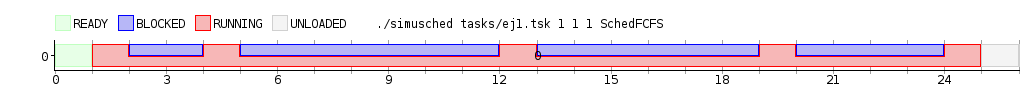
\includegraphics[width=1\columnwidth]{imagenes/ej1.png}
			\caption{\texttt{TaskBatch} corriendo con $total_cpu = 4$, $cant_bloqueos = 2$.}
		\end{center}
	\end{figure}

